% oursland2024_nn_as_nn.tex

\documentclass[11pt]{article}

% Packages
\usepackage{amsmath, amssymb}
\usepackage{graphicx}
\usepackage{natbib}
\usepackage{geometry}
\usepackage{hyperref}
\usepackage{booktabs}
\usepackage{authblk}
\usepackage{caption}
\usepackage{subcaption}  % For subfigures

% Geometry
\geometry{
    a4paper,
    left=25mm,
    right=25mm,
    top=25mm,
    bottom=25mm,
}

% Title and Author
\title{Neural Networks as Nearest Neighbors}
\author{Alan Oursland}
\affil{Independent Researcher}
\date{September 2024}

\begin{document}

\maketitle

% Abstract
\begin{abstract}
\begin{abstract}
    This paper establishes a novel connection between neural network architectures and the 
    Mahalanobis distance, a statistical measure accounting for data covariance structure. 
    We provide a robust mathematical framework bridging neural networks with this 
    statistical distance measure, demonstrating how Absolute Value (Abs) activations 
    facilitate distance-based interpretations. This distance-based 
    interpretation has the potential to enhance model robustness, improve generalization, 
    and provide more intuitive explanations of neural network decisions. 
    \end{abstract}
\end{abstract}
 
% Sections
% introduction.tex

\section{Introduction}

Neural networks have become a cornerstone of modern machine learning, achieving state-of-the-art results in various domains. Despite their success, understanding the internal workings and interpretability of neural networks remains a challenge. In this paper, we propose a novel interpretation by viewing neural networks as nearest neighbor models.

We begin by deriving mathematical connections between linear layers and Mahalanobis distances. Building on this foundation, we conduct experiments to validate our approach and compare it with traditional activation functions and nearest neighbor algorithms.

Our contributions are as follows:
\begin{itemize}
    \item We provide a mathematical framework linking neural networks to nearest neighbor methods.
    \item We demonstrate through experiments how linear nodes with absolute value activations approximate distances to cluster centers.
    \item We interpret the learned features of neural networks under this new perspective.
\end{itemize}

% The remainder of this paper is organized as follows: Section~\ref{sec:math_framework} presents the mathematical framework. Section~\ref{sec:experiment1} details the first experiment on a synthetic dataset. Section~\ref{sec:experiment2} explores experiments on the MNIST dataset. In Section~\ref{sec:interpretation}, we interpret the learned features. Section~\ref{sec:experiment3} applies the approach to the LeNet architecture. Finally, Section~\ref{sec:discussion} discusses the implications, and Section~\ref{sec:conclusion} concludes the paper.





% math_framework.tex

\section{Mathematical Framework}
\label{sec:math_framework}

In this section, we develop the mathematical foundation that connects neural networks to the Mahalanobis distance, thereby providing a framework for interpreting neural network operations through the lens of statistical distance metrics. We begin by revisiting key concepts related to Gaussian distributions and the Mahalanobis distance, followed by a detailed exploration of how neural network components, particularly linear layers and activation functions, can approximate these distance metrics. This framework not only enhances our understanding of neural network behavior but also lays the groundwork for leveraging statistical principles to improve network interpretability and training dynamics.

\subsection{Mahalanobis Distance for a Multivariate Gaussian Distribution}

A multivariate Gaussian (normal) distribution is a fundamental concept in statistics, describing a \(d\)-dimensional random vector \(\mathbf{x} \in \mathbb{R}^d\) with a mean vector \(\boldsymbol{\mu} \in \mathbb{R}^d\) and a covariance matrix \(\boldsymbol{\Sigma} \in \mathbb{R}^{d \times d}\) \citep{bishop2006pattern}. We denote this distribution as \(\mathbf{x} \sim N(\boldsymbol{\mu}, \boldsymbol{\Sigma})\).

The Mahalanobis distance quantifies the distance between a point \(\mathbf{x}\) and the mean \(\boldsymbol{\mu}\) of a distribution, while considering the covariance structure of the data \citep{mahalanobis1936generalized, demaesschalck2000mahalanobis}. It is defined as:

\begin{equation}
\label{eq:mahalanobis_distance}
D_M(\mathbf{x}) = \sqrt{ (\mathbf{x} - \boldsymbol{\mu})^\top \boldsymbol{\Sigma}^{-1} (\mathbf{x} - \boldsymbol{\mu}) }.
\end{equation}

This metric adjusts for variance across dimensions by effectively whitening the data, resulting in a spherical distance measure.

\subsection{Principal Component Analysis (PCA)}

Principal Component Analysis (PCA) is a dimensionality reduction technique that transforms data into a new coordinate system, emphasizing directions (principal components) that capture the most variance \citep{jolliffe2002principal}. When performing PCA on the covariance matrix $\boldsymbol{\Sigma}$, it is decomposed using eigenvalue decomposition:

\begin{equation}
    \label{eq:pca_decomposition}
    \boldsymbol{\Sigma} = \mathbf{V} \boldsymbol{\Lambda} \mathbf{V}^\top,
\end{equation}

where:
\begin{itemize}
    \item $\mathbf{V} = [\mathbf{v}_1, \mathbf{v}_2, \dots, \mathbf{v}_d]$ is a matrix whose columns are the orthogonal unit eigenvectors of $\boldsymbol{\Sigma}$.
    \item $\boldsymbol{\Lambda} = \text{diag}(\lambda_1, \lambda_2, \dots, \lambda_d)$ is a diagonal matrix of the corresponding eigenvalues $\lambda_i$, representing the variance along each principal component.
\end{itemize}

Substituting $\mathbf{V} \boldsymbol{\Lambda} \mathbf{V}^\top$ for $\boldsymbol{\Sigma}$ in the Mahalanobis distance equation \eqref{eq:mahalanobis_distance}, we obtain:

\begin{equation}
    \label{eq:mahalanobis_pca}
    D_M(\mathbf{x}) = \sqrt{ (\mathbf{x} - \boldsymbol{\mu})^\top \mathbf{V} \boldsymbol{\Lambda}^{-1} \mathbf{V}^\top (\mathbf{x} - \boldsymbol{\mu}) }.
\end{equation}

To further simplify, we can express the Mahalanobis distance in terms of the principal components:

\begin{align}
D_M(\mathbf{x}) &= \sqrt{ (\mathbf{x} - \boldsymbol{\mu})^\top \mathbf{V} \boldsymbol{\Lambda}^{-1} \mathbf{V}^\top (\mathbf{x} - \boldsymbol{\mu}) } \nonumber \\
&= \sqrt{ (\mathbf{V}^\top (\mathbf{x} - \boldsymbol{\mu}))^\top \boldsymbol{\Lambda}^{-1} (\mathbf{V}^\top (\mathbf{x} - \boldsymbol{\mu})) } \nonumber \\
&= \sqrt{ \sum_{i=1}^{d} \lambda_i^{-1} \left( \mathbf{v}_i^\top (\mathbf{x} - \boldsymbol{\mu}) \right)^2 } \nonumber \\
&= \left\| \lambda_i^{-1/2} \mathbf{v}_i^\top (\mathbf{x} - \boldsymbol{\mu}) \right\|_2.
\label{eq:mahalanobis_pca_l2}
\end{align}

where $\| \cdot \|_2$ denotes the Euclidean (L2) norm. 

This shows that the Mahalanobis distance can also be expressed as the L2 norm of the number of standard deviations of \(\mathbf{x}\) along each principal component.

\subsection{Connecting Neural Networks to Mahalanobis Distance}

We consider the Mahalanobis distance along a single principal component.

\begin{equation}
    \label{eq:mahalanobis_single_component}
    D_{M,i}(\mathbf{x}) = \left| \lambda_i^{-1/2} \mathbf{v}_i^\top (\mathbf{x} - \boldsymbol{\mu}) \right|,
\end{equation}

This equation projecting the centered data $(\mathbf{x} - \boldsymbol{\mu})$ onto the direction of variance defined by the principal component eigenvector and scales by the inverse square root of the eigenvalue (variance).

Let 
\begin{align}
    \mathbf{W} &= \lambda_i^{-1/2} \mathbf{v}_i^\top, \\
    \mathbf{b} &= - \lambda_i^{-1/2} \mathbf{v}_i^\top \boldsymbol{\mu}.
\end{align}

We can simplify Equation \eqref{eq:mahalanobis_single_component} to

\begin{equation}
    \label{eq:mahalanobis_linear}
    D_{M,i}(\mathbf{x}) = \left| \mathbf{W} \mathbf{x} - \mathbf{b} \right|,
\end{equation}

This is identical to the equation for a linear layer where $\boldsymbol{W}$ represents the weight matrix, $\boldsymbol{b}$ the bias vector, and the Abs function serves as the activation function.

Linear nodes with Abs activations can be interpreted as 1d Gaussians along a direction of variance with the decision boundary passing through the mean of the modelled cluster.

Extending this to all principal components, the Mahalanobis distance can be represented as a multiple linear nodes, each corresponding to a principal component, followed by an Abs activation. This layered structure inherently accounts for the covariance structure of the data, effectively 'whitening' the input.

\subsection{Non-Uniqueness of Whitening}

Calculating the Mahalanobis distance along each principal component results in a whitened data set. 

Whitening data is defined as follows:

\[
\mathbf{x}_w = \boldsymbol{\Lambda}^{-1/2} \mathbf{V}^\top (\mathbf{x} - \boldsymbol{\mu}),
\]

where \(\mathbf{x}_w\) follows a distribution \(\mathcal{N}(0, I)\).

The Mahalanobis distance can then be expressed as:

\[
D_M(\mathbf{x}_w) = \|\mathbf{x}_w\|_2.
\]

However the vectors to generate whitened data are not unique.

We can select a rotation matrix \(\mathbf{R} \in SO(n)\) such that:

\begin{align}
    D_M(\mathbf{x}_w) &= D_M(\mathbf{R} \mathbf{x}_w) \\
                      &= D_M\left( (\mathbf{R} \boldsymbol{\Lambda}^{-1/2} \mathbf{V}^\top) (\mathbf{x} - \boldsymbol{\mu}) \right) \\
                      &= D_M\left( \boldsymbol{\Lambda}^{-1/2} (\mathbf{V}^\top \mathbf{R}) (\mathbf{x} - \boldsymbol{\mu}) \right).
    \end{align}
    
The Mahalanobis distance for whitened data remains invariant under the application of rotation matrices. If we transform the rotated basis back to the original space, we end up with a whitening basis whose component vectors may not be orthogonal.

This implies that, although linear nodes can represent principal components, they are unlikely to actually learn the principal components when estimating Mahalanobis distances. Instead, they are expected to learn an basis that effectively whitens the data for use in the Mahalanobis distance estimation. However, the decision boundary of the learned hyperplane should still pass through the data mean.

\subsection{Approximating Mahalanobis Distance with Neural Networks}

Following the Abs function with another linear node allows for a summation of the principal component whitened data, leading to the following expression for the Mahalanobis distance:

\begin{equation}
    \label{eq:mahalanobis_L1}
    y = \sum \left| \mathbf{W_c} \mathbf{x} - \mathbf{b_c} \right|,
\end{equation}

L1 norms have been utilized as an effective alternative to L2 norms in various high-dimensional applications \citep{bernhardsson2018annoy}. In finite-dimensional vector spaces, all norms are equivalent up to constant factors, allowing L1 norms to bound and be bounded by L2 norms \citep{kreyszig1978introductory}. Moreover, L1 norms offer robustness to outliers, making them well-suited for training contexts with unexpected or noisy data \citep{candes2005decoding}. 

In the neural network architecture, each Abs-activated linear node computes the absolute deviation along a specific principal component direction. The subsequent summation node aggregates these deviations, thereby approximating the overall Mahalanobis distance through an L1 norm-based aggregation of L2-like components. This approach leverages the computational efficiency and robustness of L1 norms while maintaining the interpretability of Mahalanobis distance in high-dimensional spaces.

\section{Experiment 1: Single Linear Node on a 2D Gaussian}
\label{sec:experiment1}

In this experiment, we investigate whether single linear-node neural networks with either absolute value (Abs) or rectified linear unit (ReLU) activation functions can learn to approximate the Mahalanobis distance in a 2D Gaussian distribution. Specifically, we aim to determine if these simple models capture the principal components of the Gaussian distribution, as predicted by our theoretical framework.

\subsection{Methodology}

We generated a synthetic dataset from a bivariate Gaussian distribution. The dataset $X$ was used to compute the true Mahalanobis distance for each point Equation~\eqref{eq:mahalanobis_distance}. These distances served as the target outputs $y$ for training the models.

Each model consisted of a single linear unit followed by either a ReLU or Abs activation function. Weights were initialized using Xavier initialization. To ensure diverse initial conditions, we selected a random point $\mathbf{z} \in \mathbb{R}^2$ uniformly from $[-8, 8]^2$ and set the bias as:

\begin{equation} b = -\mathbf{W} \mathbf{z}, \end{equation}

so that the decision boundary (defined by $\mathbf{W} \mathbf{x} + b = 0$) passes through the point $\mathbf{z}$. This strategy ensures that the initial decision boundaries are distributed throughout the input space.

To prevent dead ReLU nodes (nodes that output zero for all inputs), we checked the initial activations and reinitialized any models where this occurred.

Setup and training parameters are summarized in Table~\ref{tab:config_params}.

\begin{table}[h]
\centering
\caption{Configuration Parameters}
\label{tab:config_params}
\begin{tabular}{ll}
\hline
Parameter & Value \\
\hline
Activation Functions & ReLU, Abs \\
Loss Function & Mean Squared Error (MSELoss) \\
Optimizer & SGD \\
Learning Rate & 0.001 \\
Epochs & 200 \\
Momentum & 0.9 \\
Weight Initialization & Xavier Initialization \\
Bias Initialization & $b = -\mathbf{W} \mathbf{z}$, $\mathbf{z} \sim \mathcal{U}([-8,8]^2)$ \\
Number of Models & 300 per activation function \\
Number of Data Points & 1024 \\
Mean Vector $\boldsymbol{\mu}$ & $[3.0, 2.0]^\top$ \\
Covariance Matrix $\boldsymbol{\Sigma}$ & $\begin{bmatrix} 2.0 & -1.0 \\ -1.0 & 1.0 \end{bmatrix}$ \\
\hline
\end{tabular}
\end{table}

\subsection{Objectives and Hypotheses}

Based on our theoretical framework, we hypothesize the following:

\begin{enumerate} 
    \item \textbf{Abs Activation Hypothesis}: Models using the Abs activation function will learn to approximate the Mahalanobis distance by aligning their weights the largest principal component of the Gaussian distribution. This alignment should result in lower error compared to models using ReLU activations.
    \item 
    \item \textbf{ReLU Activation Hypothesis}: Models using the ReLU activation function are less likely to align with the principal components due to the asymmetry of the ReLU function, potentially resulting in higher error. However, studying their solution space may provide insights into how ReLU models approximate the distance function.
\end{enumerate}

\subsection{Results and Discussion}

\subsubsection{Visualization of Learned Weights}

To analyze the learned models, we visualized the weights $\mathbf{W}$ by representing them as vectors originating from the projection of the mean vector $\boldsymbol{\mu}$ onto the model's decision boundary. Specifically, for each model, we:

\begin{enumerate} \item Calculated the point $\mathbf{p}$ where the decision boundary intersects the line passing through $\boldsymbol{\mu}$ and perpendicular to the decision boundary.
    \item Represented the weight vector $\mathbf{W}$ as an arrow originating from $\mathbf{p}$.

    \item Scaled the weight vectors for visualization purposes but maintained their orientation to reflect the learned directions.
    
\end{enumerate}

This visualization allows us to assess how the models' learned weights align with the principal components of the data distribution.

\begin{figure}[h]
    \centering
    \begin{subfigure}[b]{0.48\textwidth}
        \centering
        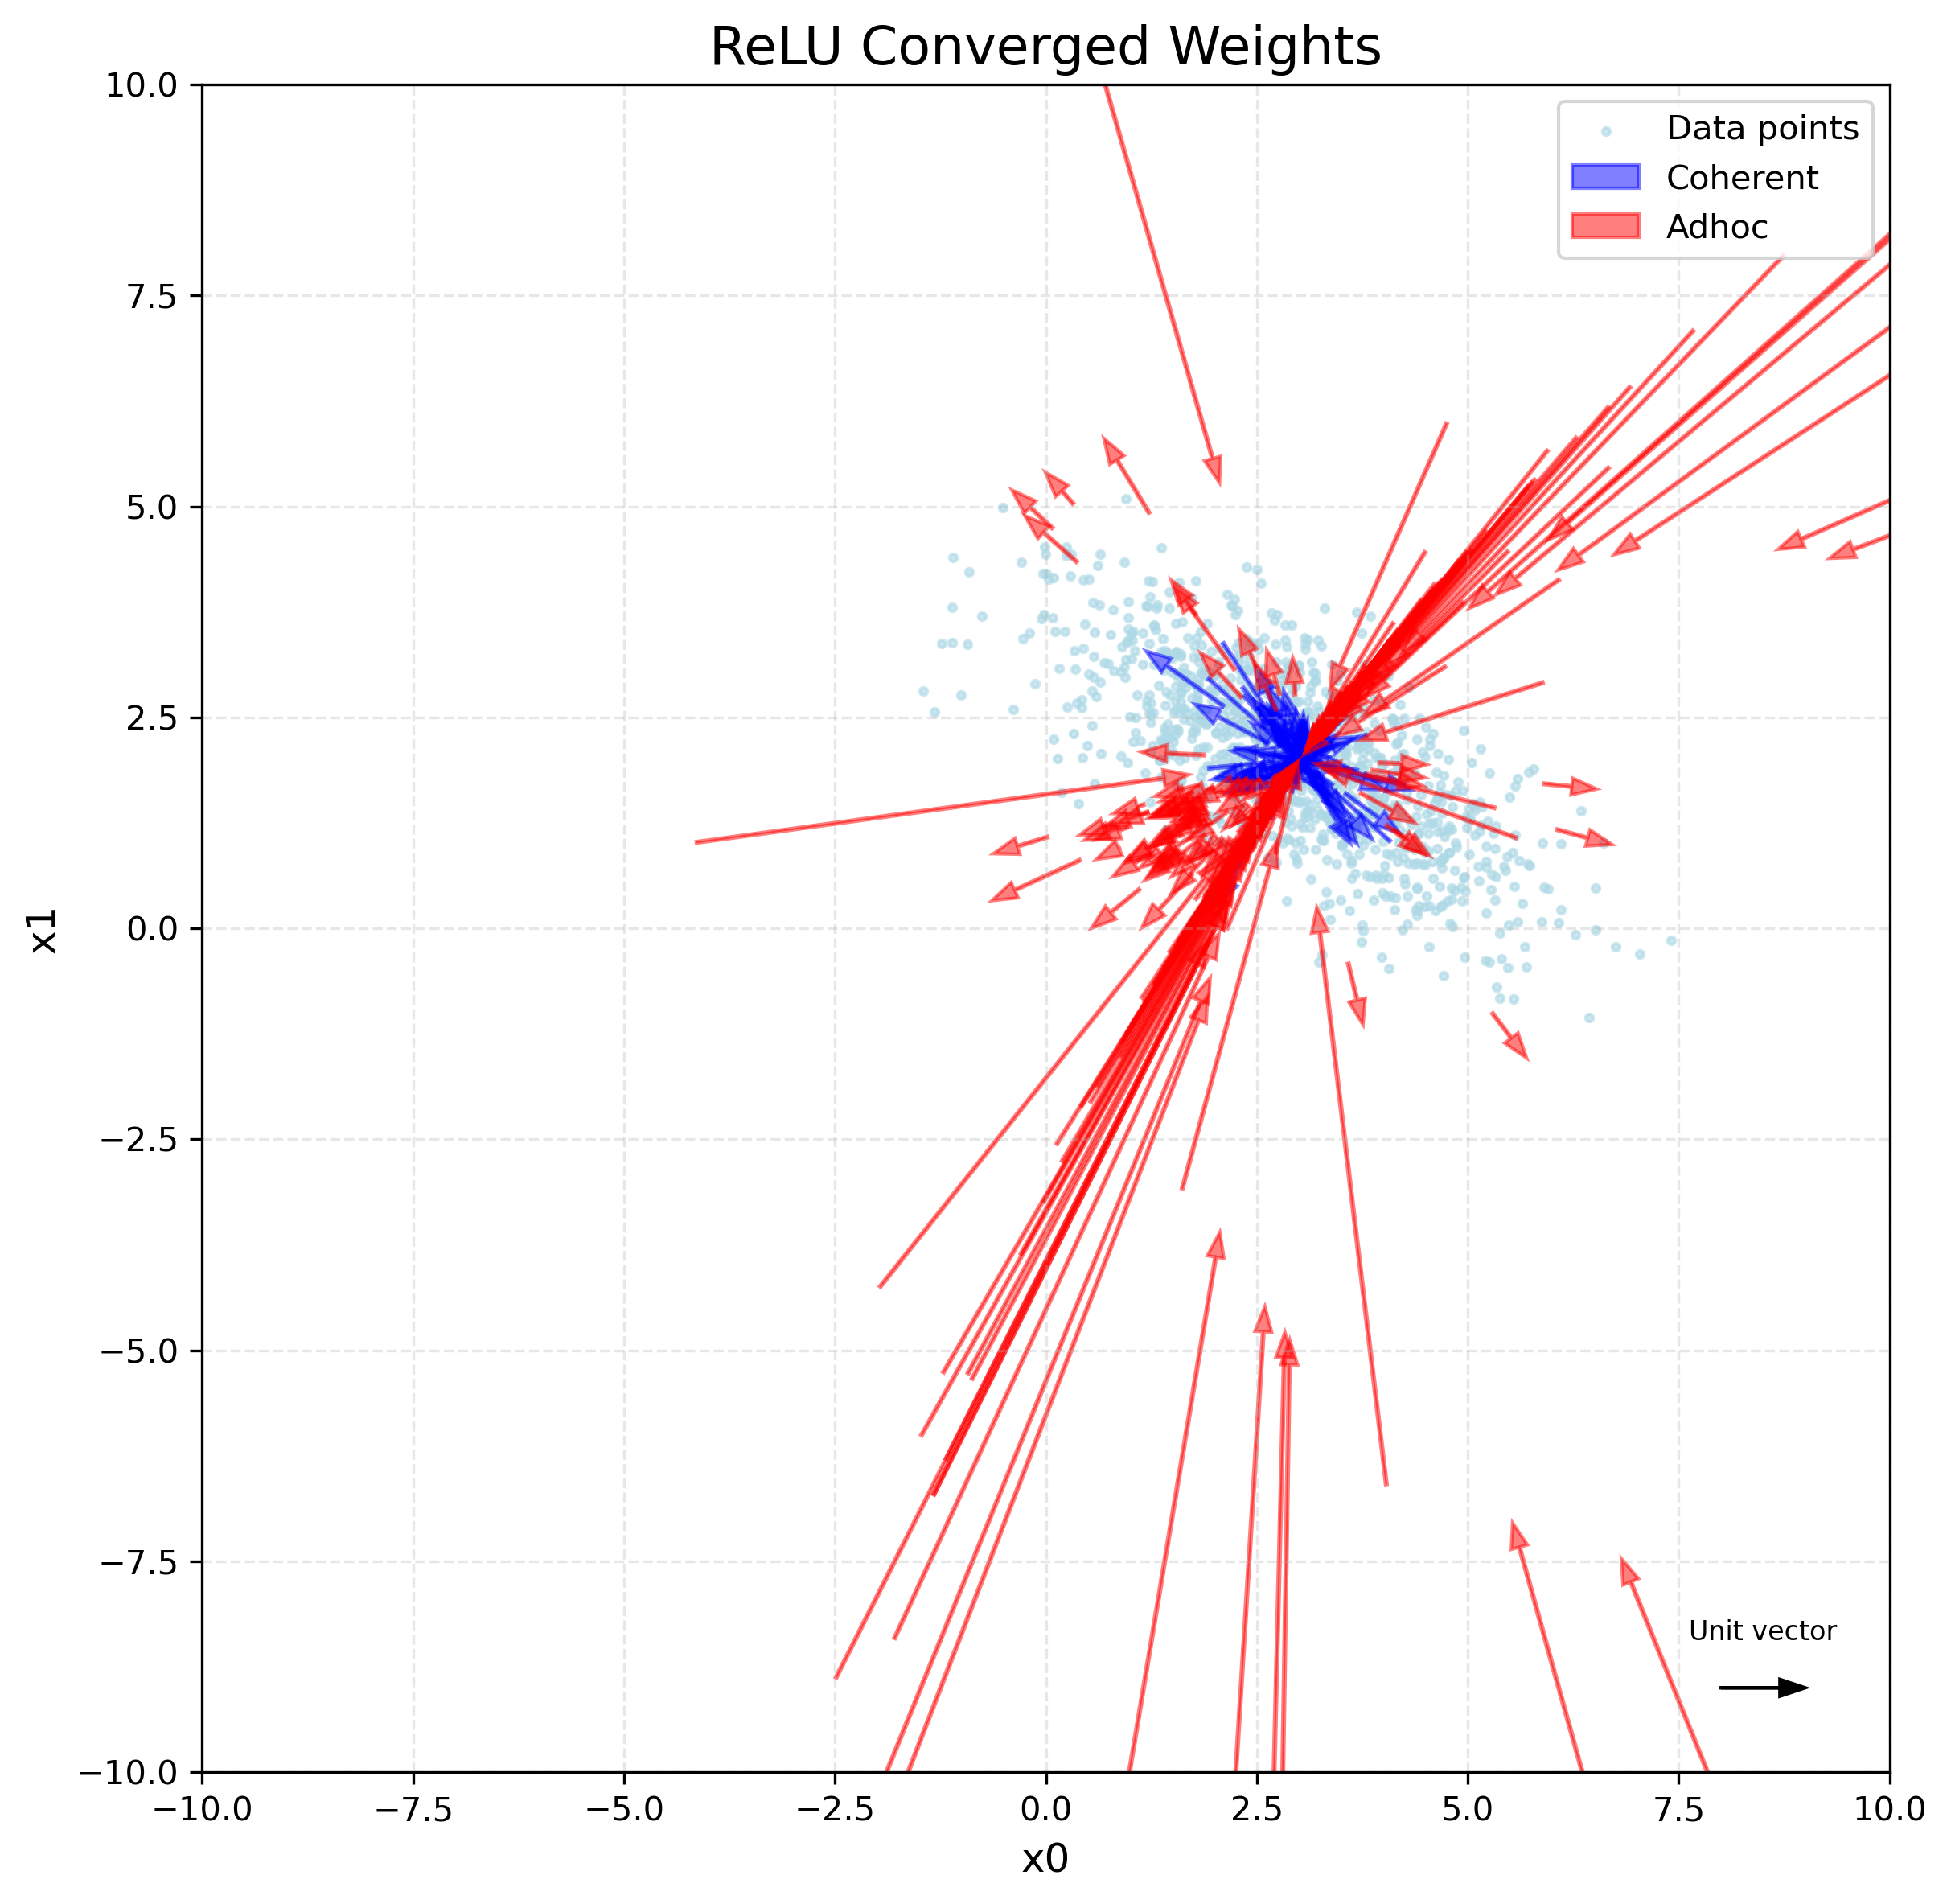
\includegraphics[width=\linewidth]{converged_states_relu.png}
        \caption{ReLU Activation}
        \label{fig:converged_relu}
    \end{subfigure}
    \hfill
    \begin{subfigure}[b]{0.48\textwidth}
        \centering
        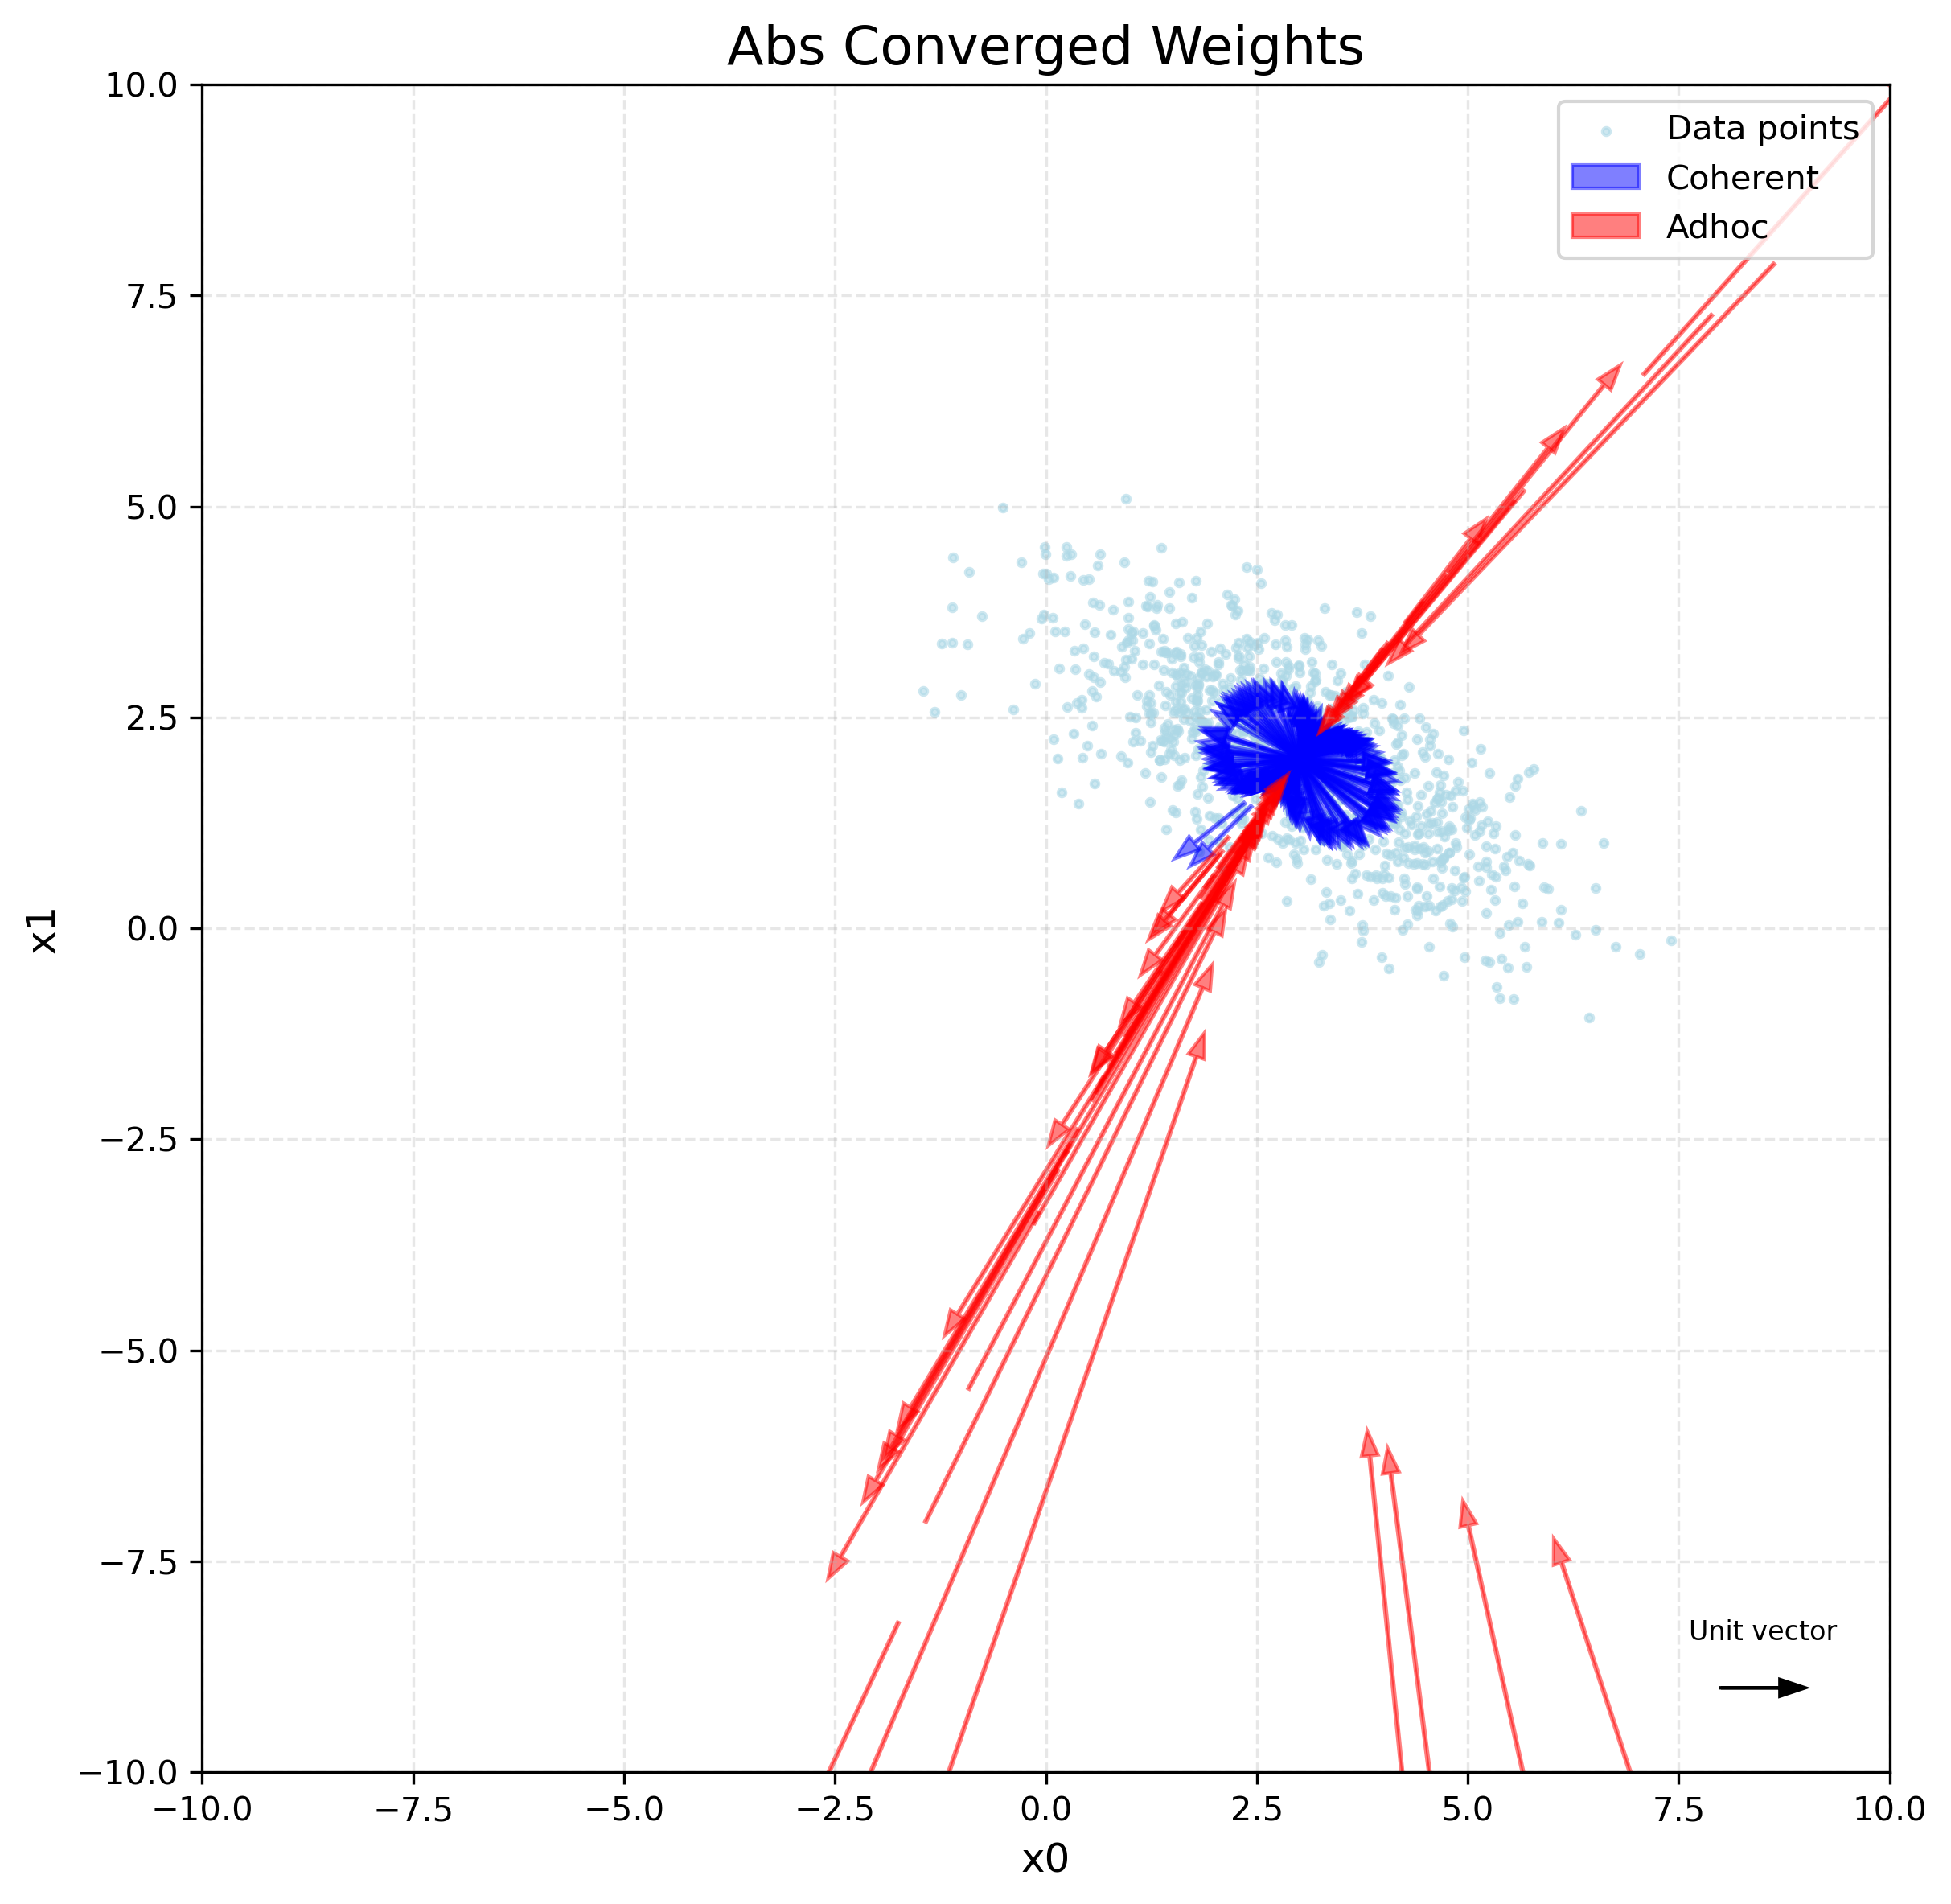
\includegraphics[width=\linewidth]{converged_states_abs.png}
        \caption{Abs Activation}
        \label{fig:converged_abs}
    \end{subfigure}    
    \caption{Converged states for ReLU and Abs activations. The blue dots represent the 2D Gaussian data points. Arrows represent the learned weight vectors originating from the projection of $\boldsymbol{\mu}$ onto the decision boundary. Blue arrows indicate Coherent solutions, and red arrows indicate Adhoc solutions.}
    \label{fig:converged_states}
\end{figure}
    
\subsubsection{Solution Classes: Coherent vs.\ Adhoc}

Upon analysis, we observed that the solutions could be classified into two categories:

\begin{itemize} 
    \item \textbf{Coherent Solutions}: Models where the decision boundary intersects the Gaussian mean $\boldsymbol{\mu}$. These models tend to align with the statistical properties of the data, potentially capturing the principal components. We classified a model as Coherent if the distance between $\boldsymbol{\mu}$ and the decision boundary was less than a small threshold $\epsilon$.
    
    \item \textbf{Adhoc Solutions}: Models where the decision boundary does not intersect $\boldsymbol{\mu}$. These models approximate the target function through other means and may not have an obvious interpretation with respect to the data's statistical properties.
\end{itemize}

\subsubsection{Quantitative Results}

Table~\ref{tab:ex1_stats} summarizes the results of the experiment. The Mean Squared Error (MSE) is reported for both activation functions, along with the counts of models in each solution class.

\begin{table}[h]
    \centering
    \caption{Single Linear Node Results}
    \label{tab:ex1_stats}
    \begin{tabular}{|l|c|c|}
    \hline
    Metric & ReLU & Abs \\
    \hline
    Error & 1.090 & 0.468 \\
    Coherent Error & 0.976 & 0.455 \\
    Adhoc Error & 0.822 & 0.523 \\
    Coherent Count & 4 & 243 \\
    Adhoc Count & 214 & 57 \\
    Dead Count & 82 & 0 \\
    \hline
    \end{tabular}
    \end{table}

\subsubsection{Analysis of Results}

\paragraph{ReLU Activation Models}

As shown in the left image of Figure~\ref{fig:converged_states}, most ReLU models ($214$ out of $300$) resulted in Adhoc solutions. These models tended to align their weights with the dimension of least variance, possibly attempting to minimize error estimating an overall average. The average MSE for ReLU models was higher than that of Abs models, and the Coherent ReLU models had higher error than their Adhoc counterparts.

\paragraph{Abs Activation Models}

The right image in Figure~\ref{fig:converged_states} illustrates the converged states for models with Abs activation. The majority of these models ($243$ out of $300$) produced Coherent solutions, with decision boundaries intersecting near the Gaussian mean. These models exhibited lower average MSE compared to Adhoc Abs models, confirming our hypothesis that Abs activations effectively approximate the Mahalanobis distance by aligning with a mixture of principal components.

However, the Coherent Abs models did not align the largest principal component. While the decision boundary comes very close to the cluster mean, the weights seem to express a mixture of components, as expressed in Equation~\eqref{eq:mixture_pcs}:

\begin{equation} \label{eq:mixture_pcs} \mathbf{W} = \sum_{i=1}^d \alpha_i \mathbf{v}_i^\top, \end{equation}

where $\mathbf{v}_i$ are the principal components and $\alpha_i$ are weighting coefficients. 

The displayed vectors $v / |v|^2|$, seem to form an ellipse or a pair of circles suggesting that $\ell_2(\alpha)=1$ or perhaps that the foci of the Gaussian ellipse have some relationship to the gradient. The exact relationship requires further study. There may be a numerical instability around the direction of least variance that causes the decision boundaries to be ejected from the cluster.

Some of the Adhoc Abs solutions behaved like a ReLU because the Abs function on received inputs on only a single side of the decision boundary. 

\subsubsection{Observations on Initialization and Activation Functions}

The initial weights did not show a clear pattern predicting the solution class into which a model would fall. However, the behavior of the models highlights the importance of the activation function and initialization:

\begin{itemize} 
    \item \textbf{Abs Models Functioning Like ReLU}: The modes where Abs acts like ReLU suggests that proper initialization is crucial for Abs models to capture both sides of the data distribution.
    \item \textbf{ReLU Models Aligning with Least Variance Direction}: The ReLU models often aligned their weights with the smallest principal component, minimizing output the variance across data points. The models are trying to return a constant value, presumably the mean of the target values.
    \item \textbf{Importance of Decision Boundary Placement}: Ensuring that the decision boundary intersects the data cluster increases the likelihood of a model learning a Coherent solution, particularly for Abs activations.
\end{itemize}

\subsection{Conclusion and Next Steps}

The Abs models do not learn principal components directly as we theorized. Instead we discovered a surprising fact about the power of linear units: A single linear unit can estimate the Mahalanobis distance for any dimension Gaussian through principal component mixing.

The findings also reveal the importance of initialization strategies. Abs models that failed to intersect the data cluster tended to behave like ReLU models, resulting in higher error and Adhoc solutions. This suggests that initializing the bias to ensure the decision boundary passes through the data cluster can improve model performance.

\subsection{Data Sampling Initialization}

To address the observations from the initial experiment regarding the importance of the decision boundary intersecting the data cluster, we explored a novel initialization strategy for the bias $b$. Instead of selecting a random point $\mathbf{z}$ from the uniform distribution over $[-8, 8]^2$, we now initialize $b$ using a randomly selected data point $\mathbf{x}_0$ from the dataset $X$. Specifically, we set:

\begin{equation}
b = -\mathbf{W} \mathbf{x}_0,
\end{equation}

ensuring that the initial decision boundary passes through a point within the data cluster. This approach increases the likelihood that the model will capture variations on both sides of the decision boundary, particularly for models using the Abs activation function.

Other than this modification to the bias initialization, all other parameters and settings remain the same as in the initial experiment (see Table~\ref{tab:config_params}).

\subsubsection{Results and Discussion}

Table~\ref{tab:data_init_results} summarizes the results of the experiment using the data sampling initialization strategy.

\begin{table}[h]
    \centering
    \caption{Results with Data Sampling Initialization}
    \label{tab:data_init_results}
    \begin{tabular}{|l|c|c|}
    \hline
    Metric & ReLU & Abs \\
    \hline
    Average MSE (All Models) & 0.833 & 0.407 \\
    Average MSE (Coherent Models) & 1.165 & 0.396 \\
    Average MSE (Adhoc Models) & 0.660 & 0.541 \\
    Number of Coherent Models & 93 & 277 \\
    Number of Adhoc Models & 203 & 23 \\
    Number of Dead Models & 4 & 0 \\
    \hline
    \end{tabular}
\end{table}

Compared to the initial experiment, the data sampling initialization significantly increased the number of Coherent solutions for both activation functions, especially for the Abs models. Specifically, the number of Coherent Abs models increased from 243 to 277 out of 300, while the number of Adhoc Abs models decreased correspondingly.

For the ReLU models, the number of Coherent solutions also increased from 4 to 93, and the number of dead nodes decreased dramatically from 82 to 4. This suggests that initializing the bias using a data point from the dataset effectively activates more ReLU models, allowing them to participate in learning.

\paragraph{Analysis of Abs Models}

The Abs models benefited significantly from the data sampling initialization. The increase in Coherent models indicates that more models had decision boundaries intersecting the data cluster, allowing them to capture variations on both sides of the mean. This led to a slight improvement in the average MSE for Coherent Abs models (from 0.455 to 0.396).

The reduction in the number of Adhoc Abs models further supports the effectiveness of the initialization strategy. With fewer models behaving like ReLU due to all data points being on one side of the decision boundary, the overall performance of the Abs models improved.

\paragraph{Analysis of ReLU Models}

The data sampling initialization led to a significant decrease in the number of dead ReLU nodes, from 82 down to 4. Most of the nodes that were previously dead became Coherent nodes, increasing the number of Coherent ReLU models from 4 to 93 out of 300. This suggests that initializing the bias using data points effectively activates more ReLU models, allowing them to contribute to learning.

While the number of Coherent ReLU models increased, their average MSE also increased (from 0.976 to 1.165). This indicates that although more ReLU models had decision boundaries intersecting the data cluster, they were still limited by the asymmetry of the ReLU activation function, which hinders their ability to approximate the Mahalanobis distance effectively.

The average MSE for Adhoc ReLU models decreased from 0.822 to 0.660. This decrease is noteworthy, but the exact reason is unclear. It may be due to the data sampling initialization producing better Adhoc models; however, further investigation is needed to confirm this. Therefore, we simply note this observation without proposing a specific cause.

\subsubsection{Conclusion of Data Sampling Initialization Experiment}

For the Abs models, this initialization strategy reinforced their ability to approximate the Mahalanobis distance through principal component mixing, as more models aligned their weights with a mixture of principal components.

For ReLU models, while there was an increase in Coherent solutions, their inherent limitations due to the activation function's asymmetry remained evident. 

The data sampling initialization strategy proved effective in increasing the number of Coherent solutions. By ensuring that the decision boundary intersects the data cluster, the models are better positioned to learn representations that capture the statistical properties of the data.

\subsection{Overall Conclusion of Experiment 1}

Experiment 1 reveals that:

\begin{itemize}
    \item Single linear nodes with Abs activation can approximate the Mahalanobis distance of a multivariate Gaussian distribution by learning a mixture of principal components.
    \item We observe two classes of solutions: Coherent units represent deep statistical properies of the data. Adhoc units find solutions that are not deeply grounded in statistical properties.
    \item Initialization strategies that ensure the decision boundary intersects the data cluster enhance the likelihood of models converging to Coherent solutions.
\end{itemize}

Coherent solutions have lower error with Abs. However, this problem was designed for the Abs node to do well on. Coherent solutions in ReLU have higher error, however Abs can be replicated with two ReLU nodes. Additionally, ReLU nodes can also express a signed Mahalanobis distance over [-d..d] using [0..2d] with the next layer accounting for the zero offset. In practice there should not be a huge performance difference between Abs and ReLU.

Adhoc solutions seem to minimize output variance, perhaps attempting to calculate a mean of the target data.

While our initialization strategy increases the change of Coherent features, we don't know that Coherent features are actually beneficial in full models. The next set of experiments, we will investigate whether the benefits of Coherent features and Abs activations persist when applied to the MNIST dataset. This will help determine the practicality and scalability of our approach in more complex scenarios.
% experiment2.tex

\section{Experiment 2: Shallow Networks on MNIST}
\label{sec:experiment2}

TBD: This experiment trains two layer networks on MNIST using Abs and ReLU with and without the proposed initialization strategy. It also uses kMeans to train a nearest neighbor model to compare performance.

Experiment 2 explores the practicality of our distance metric interpretation of neural networks. Expanding from simpler models in Experiment 1, we train a two-layer feedforward network on the MNIST handwritten digit dataset. This experiment tests whether the Abs activation function and bias sampling improve performance in more complex, real-world tasks. We also interpret the linear nodes' representation using the L1 Mahalanobis distance framework.

Interpretation in Experiment 1 relied on the data representation ground truth. We no longer have that with MNIST. We introduce new techniques to distinguish between the Coherent and Adhoc representation classes that were identified in Experiment 1. We also find the mean input for each hidden node that represents a canonical reprsentation of the feature that node selects. We test whether an increase in Coherent nodes corresponds to improved model performance.


\subsection{Methodology}

We train a two-layer feedforward neural network on MNIST. Each layer is followed by either a ReLU or Abs activation function. The output layer also includes an activation function to ensure it functions as a distance metric, aligning with our presented theory. Weights are initialized He Normal Initialization. Bias initialization is tested between zeroing and data sampling, as introduced in Experiment 1.

We used cross entropy loss (CEL) as the model criterion. CEL expects the larger outputs to indicate class membership, but our distance metric framing treats smaller distances as indicating membership. To adapt our model to CEL, we negate the outputs of the final activation function.

We train ten models for each experimental condition.

The remaining model parameters are outlined in Table~\ref{tab:config_params_2}.

\begin{table}[h]
\centering
\caption{Configuration Parameters for Experiment 2}
\label{tab:config_params_2}
\begin{tabular}{ll}
\hline
Parameter & Value \\
\hline
Activation Functions & ReLU, Abs \\
Loss Function & CrossEntropyLoss \\
Optimizer & SGD \\
Epochs & 50 \\
Learning Rate & 0.001 \\
Momentum & 0.9 \\
Batch Size & 64 \\
Hidden Layer Size & 128 \\
Output Layer & Negated activation function \\
Weight Initialization & He Normal Initialization \\
Bias Initialization & Random or Sampled from Data \\
Dataset & MNIST (60,000 training samples, 10,000 test samples) \\
\hline
\end{tabular}
\end{table}

\subsection{Objectives and Hypotheses}

Building on our findings from Experiment 1, we hypothesize the following for Experiment 2:

\begin{itemize}
    \item \textbf{Abs vs. ReLU Hypothesis}: Abs and ReLU will perform similarly. Before the activation function is applied, the Abs node represents variance over \([- \delta .. + \delta]\), while the ReLU node represents variance over \([0 .. 2 \delta]\). Both should yield comparable overall performance despite these differences.
    
    \item \textbf{Bias Sampling Hypothesis}: Bias sampling continues to increase the number of Coherent features, even in more complex models like MNIST. This strategy should lead to better alignment of the network’s nodes with significant data clusters, improving both interpretability and model performance.
    
    \item \textbf{Coherent Features Hypothesis}: Models with a higher proportion of Coherent features will perform better than those with more Adhoc features. Coherent features align with meaningful clusters, leading to improved model generalization and accuracy.
    
    \item \textbf{Feature Interpretability Hypothesis}: Interpreting linear nodes as outputting distance metrics simplifies the understanding of the features that these nodes select, making the model’s internal structure easier to interpret.
\end{itemize}

\subsection{Results and Discussion}

\subsubsection{Performance Results}

Table~\ref{tab:ex2_results_table} summarizes the performance metrics across the different experimental conditions. We report the average accuracy, precision, recall, F1 score, and test error, along with the minimum and maximum accuracy to give a sense of variability across the ten models trained for each condition. We also include metrics for model diversity to measure the number of differing predictions between models within the same condition.

\begin{table}[h]
    \centering
    \caption{Performance Results for Experimental Conditions}
    \label{tab:ex2_results_table}
    \begin{tabular}{l|c|c|c|c}
    \hline
    Metric & ReLU & ReLU + Bias Sampling & Abs & Abs + Bias Sampling \\
    \hline
    Accuracy (Avg) & 0.9773 & 0.9770 & 0.9749 & 0.9773 \\
    Accuracy (Min) & 0.9759 & 0.9756 & 0.9554 & 0.9728 \\
    Accuracy (Max) & 0.9785 & 0.9779 & 0.9799 & 0.9795 \\
    Precision & 0.9772 & 0.9769 & 0.9750 & 0.9772 \\
    Recall & 0.9771 & 0.9768 & 0.9747 & 0.9771 \\
    F1 Score & 0.9771 & 0.9768 & 0.9748 & 0.9771 \\
    Test Error & 0.0747 & 0.0757 & 0.0855 & 0.0754 \\
    Avg Error Count & 227.0 & 230.3 & 250.9 & 227.1 \\
    Unique Errors & 509 & 509 & 805 & 617 \\
    Consistent Errors & 70 & 79 & 47 & 40 \\
    Voting Errors & 213 & 215 & 205 & 204 \\
    L2 Errors & 188 & 185 & 163 & 163 \\
    \hline
    \end{tabular}
    \end{table}
    
Figure~\ref{fig:ex2_training_test_error} presents two graphs: one showing the average training error and another showing the average test error for each configuration, displayed side by side. These curves provide insight into the learning dynamics and generalization performance of the models.


\begin{figure}[h]
    \centering
    % Placeholder for training and test error plots
    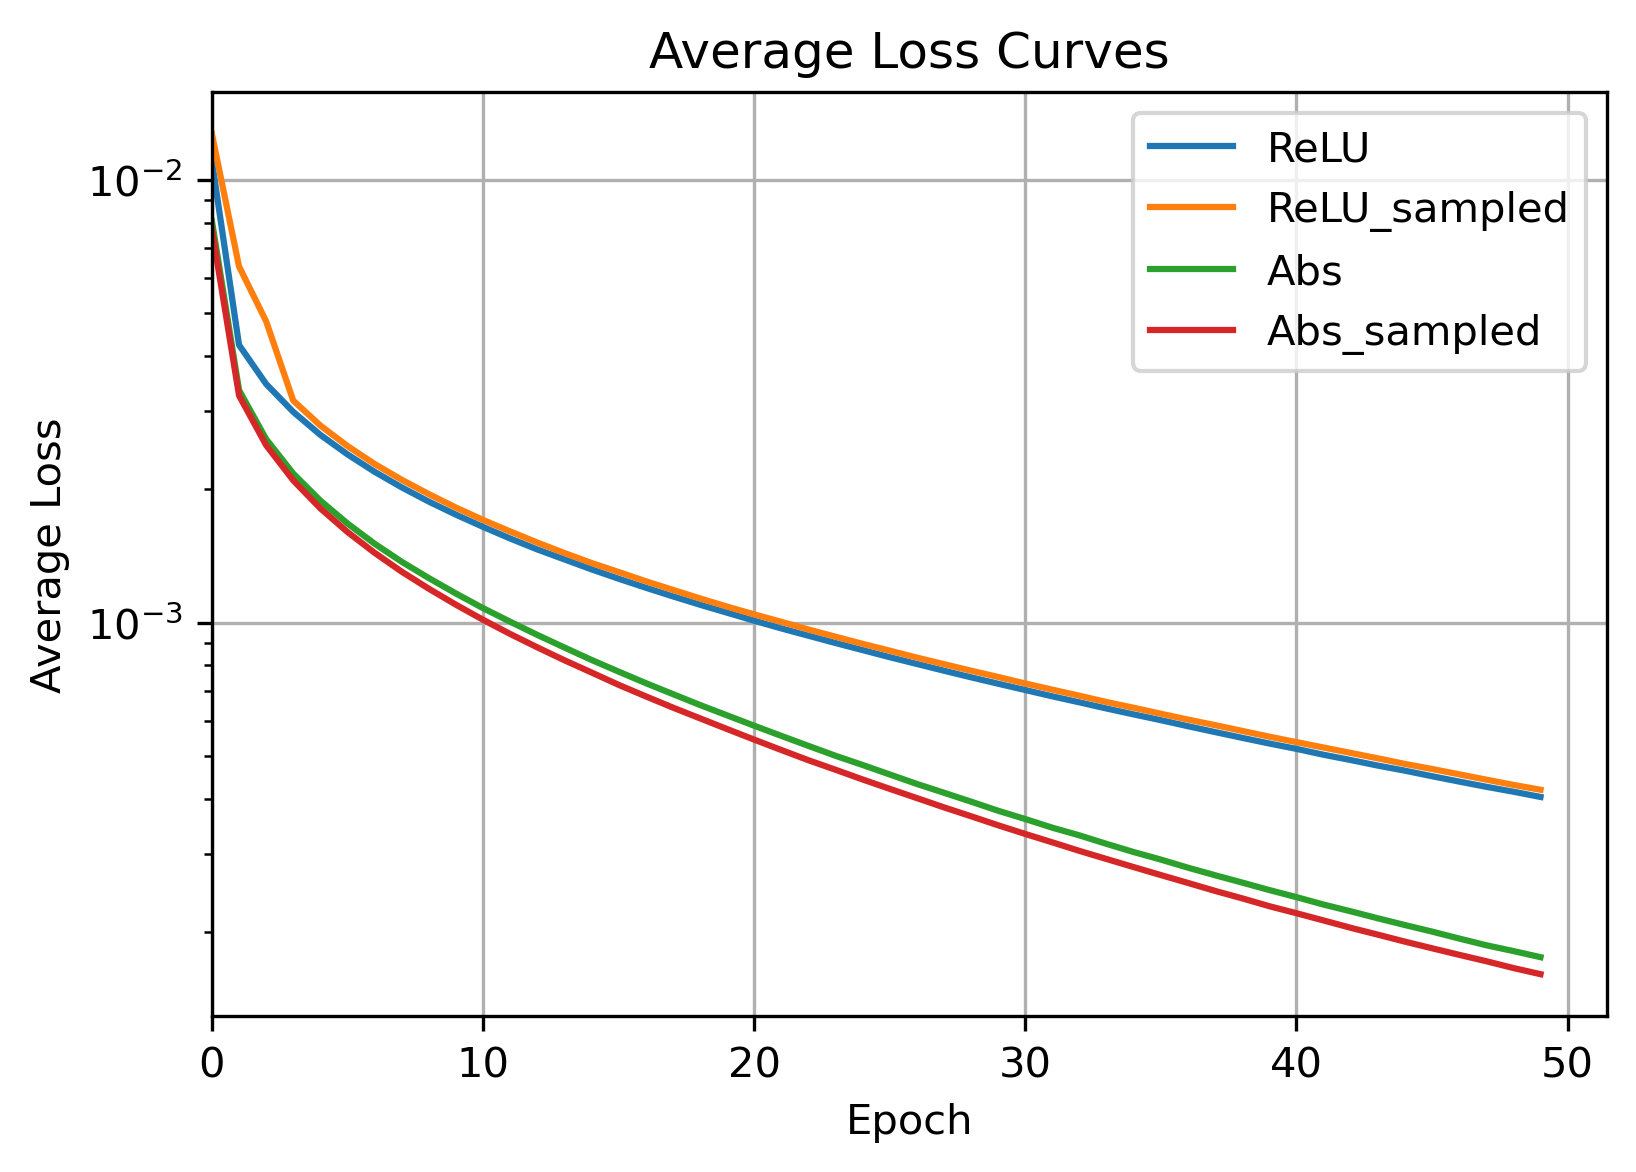
\includegraphics[width=0.45\textwidth]{ex2_training_error.png}
    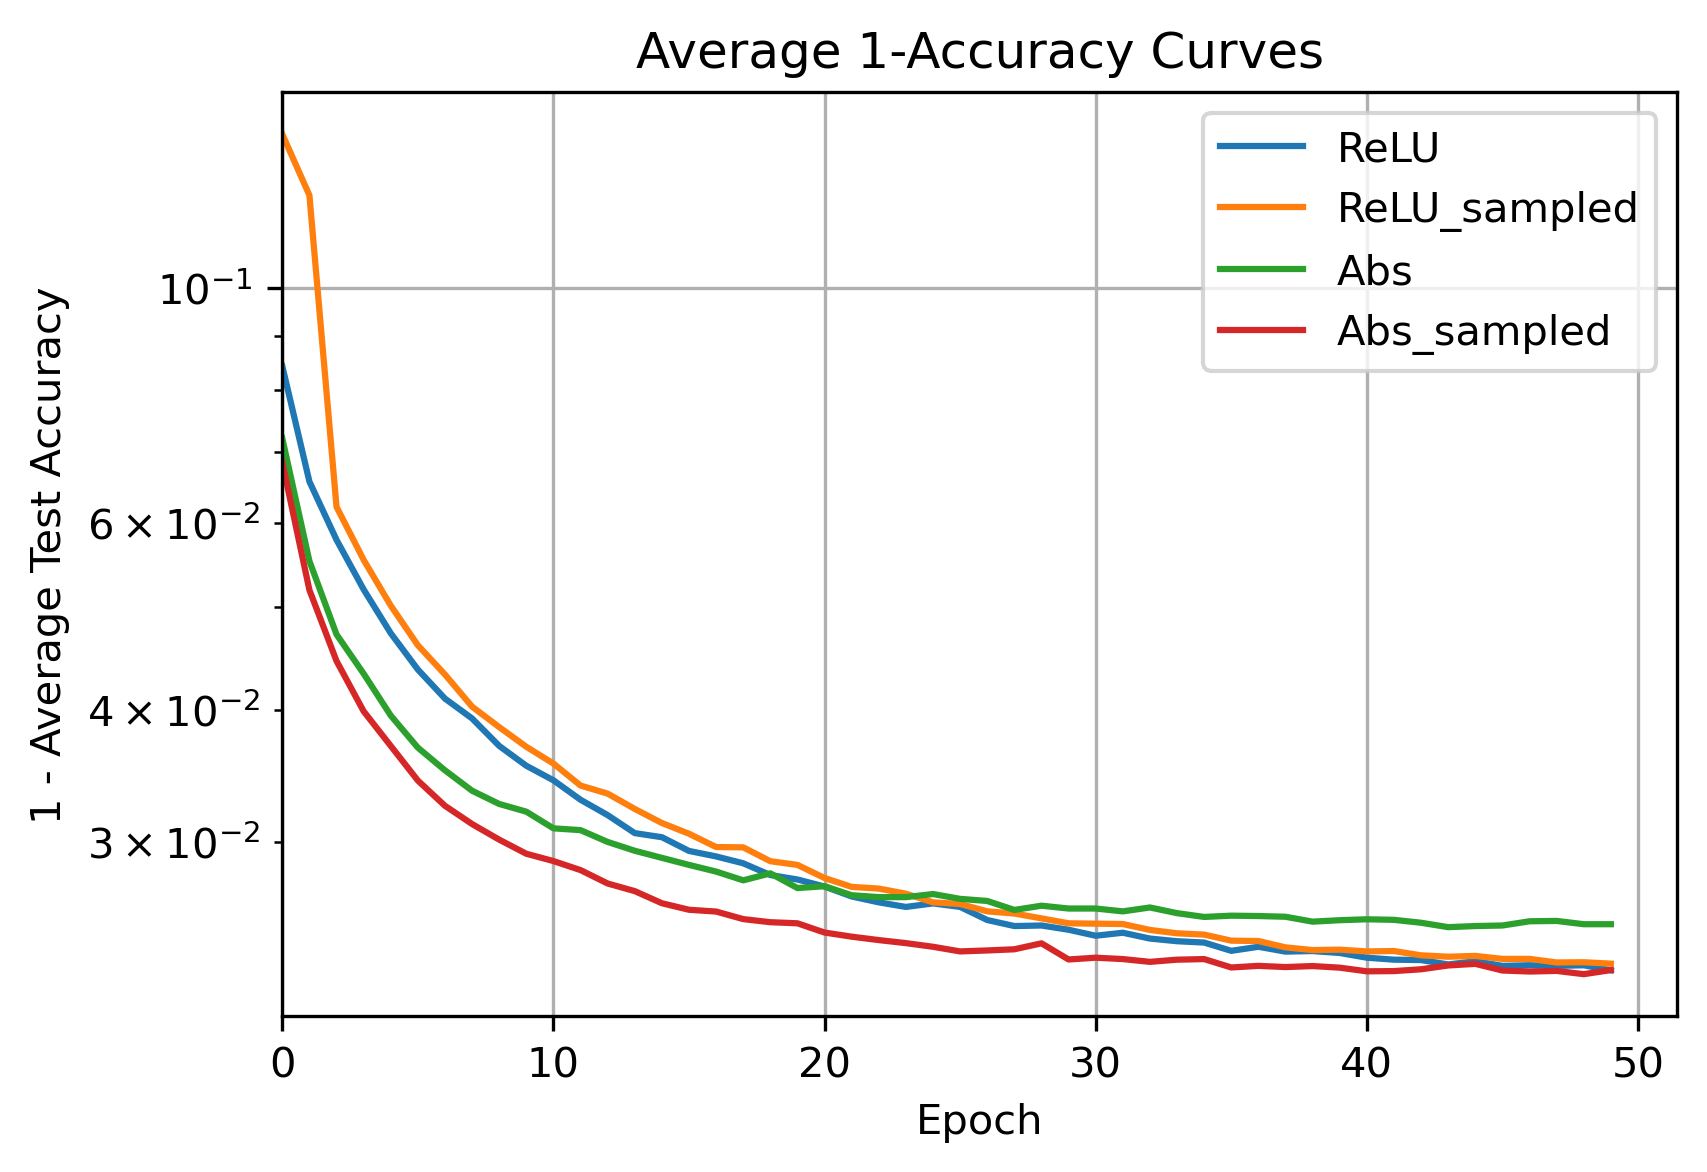
\includegraphics[width=0.45\textwidth]{ex2_test_accuracy.png}
    \caption{Training and test error curves for each experimental condition. The left plot shows the average training error, while the right plot shows the average test error. Both curves are averaged over the ten models trained for each condition.}
    \label{fig:ex2_training_test_error}
\end{figure}


\subsection{Results and Discussion}
\label{sec:results_discussion}

The performance metrics summarized in Table~\ref{tab:ex2_results_table} and Figure~\ref{fig:ex2_training_test_error} provide comprehensive insights into the effectiveness and diversity of the trained models under different experimental conditions. Each metric is averaged over ten trained models per configuration, ensuring robust statistical significance.

\paragraph{Accuracy and Performance Metrics}

All experimental configurations achieved high average accuracy on the MNIST dataset, ranging from \textbf{97.0\%} to \textbf{97.73\%}, indicating strong overall performance. Specifically, both ReLU and Abs activation functions with bias sampling attained an average accuracy of \textbf{97.73\%}. In contrast, Abs-activated models without bias sampling achieved a slightly lower average accuracy of \textbf{97.49\%}, accompanied by a broader accuracy range from \textbf{95.54\%} to \textbf{97.99\%}. This wider range for Abs without bias sampling suggests greater variability in feature learning across different training runs, potentially indicating underfitting. The higher variability is further supported by the increased number of unique errors (805) in Abs models without bias sampling compared to ReLU models (509), highlighting diverse feature representations that may not consistently capture the underlying data structure.

Precision, Recall, and F1 Score metrics are closely aligned with the observed accuracy trends. Abs-activated models without bias sampling demonstrate slightly lower Precision (\textbf{97.50\%}), Recall (\textbf{97.47\%}), and F1 Score (\textbf{97.48\%}) compared to ReLU configurations (\textbf{Precision}: 97.72\%, \textbf{Recall}: 97.71\%, \textbf{F1 Score}: 97.71\%). This minor discrepancy aligns with the broader accuracy range and higher unique error counts, indicating that while Abs models are effective, their varied feature learning may introduce inconsistencies in classification.

\paragraph{Model Diversity Metrics}

The model diversity metrics offer valuable perspectives on the consensus and variability among the trained models. Abs models without bias sampling exhibit a significantly higher number of unique errors (805), indicating that a larger number of test data points were misclassified by at least one model. In comparison, ReLU models recorded 509 unique errors, and Abs models with bias sampling had 617 unique errors. This high unique error count in Abs models without bias sampling suggests that these models are learning a more diverse set of features, capturing varied aspects of the data but at the cost of consistency across different training runs.

Consistent errors, defined as data points misclassified by all models within a configuration, remain relatively low across all conditions. Abs models with bias sampling recorded the fewest consistent errors (40), whereas ReLU models without bias sampling had the highest count (79). This indicates that bias sampling effectively reduces systematic misclassifications, promoting greater alignment with significant data clusters and enhancing overall model reliability.

Voting Errors, representing the number of data points misclassified by five or more models, are comparable across all configurations, ranging from 204 to 215. This similarity suggests that ensemble methods would encounter similar levels of misclassification regardless of activation function or initialization strategy \cite{dietterich2000ensemble}. Additionally, L2 Errors, which assess the distance metric predictions by computing the L2 norm of the prediction vectors, remain consistent across all experimental conditions (163-188), indicating stable distance-based representations.

\paragraph{Implications for Hypotheses}

The experimental results align with the proposed hypotheses in several ways:

\begin{itemize}
    \item \textbf{Abs vs. ReLU Performance}: Abs and ReLU activations exhibit similar average accuracies when bias sampling is employed. However, Abs activations without bias sampling show greater variability and higher unique error counts, supporting the hypothesis that Abs can capture diverse features but may require effective initialization to maintain consistency.
    
    \item \textbf{Bias Sampling Effectiveness}: The bias sampling initialization strategy consistently enhances model performance and reduces unique errors, particularly for Abs activations. This supports the hypothesis that bias sampling promotes better alignment with significant data clusters, thereby improving both interpretability and model performance.
    
    \item \textbf{Model Diversity and Underfitting}: The increased accuracy range and unique errors in Abs models without bias sampling suggest potential underfitting, as these models may benefit from additional hidden nodes to represent a more comprehensive set of features. This observation aligns with the hypothesis that higher model diversity can capture varied data aspects but may introduce inconsistencies.
\end{itemize}

Overall, Experiment 2 demonstrates that while both Abs and ReLU activation functions are effective in training shallow networks on the MNIST dataset, the combination of Abs activations with bias sampling initialization offers enhanced performance consistency and interpretability. The observed model diversity metrics highlight the trade-offs between feature richness and classification consistency, guiding future architectural and initialization strategies for optimizing neural network performance.


% Present the results comparing Abs and ReLU activations, as well as comparisons with K-means and Gaussian nearest neighbor implementations.


% interpretation.tex

\section{Interpretation of Learned Features}
\label{sec:interpretation}

TBD: This section uses the models trained the the previous experiment, interprets the linear nodes as Gaussian and finds the mean value. These are compared to the means used to build the kMeans NN model.

\subsection{Extracting Expected Values}

We calculated the expected value (mean) for each node's corresponding 1D Gaussian to interpret the learned features.

% Discuss the methodology and findings.

\subsection{Visualization}

% Include figures and explanations of the learned features, highlighting how they correspond to cluster centers.


% experiment3.tex

\section{Experiment 3: Application to LeNet on MNIST}
\label{sec:experiment3}

TBD: This experiment trains LeNet on MNIST using ReLU and Abs and compares performance.

\subsection{Modifying LeNet Architecture}

We adapted the LeNet architecture by replacing traditional activation functions with absolute value activations.

% Describe the modifications and rationale.

\subsection{Training and Evaluation}

% Present the training procedure and results, comparing the modified LeNet with the standard version.


% discussion.tex

\section{Implications and Discussion}
\label{sec:discussion}

We discuss implications, potential impact and future work of this reframing of linear layers in neural networks. While this paper provides a robust theoretical foundation for interpreting neural networks through Mahalanobis distance and Abs activation functions, it does not include empirical results. Future work will involve validating these theoretical insights with empirical data to further assess their applicability and performance in real-world scenarios.

\subsection{Expected Value Interpretation}

The concept of expected value or mean is fundamental in statistics and machine learning, providing a central tendency that characterizes a distribution. In the context of neural networks, identifying an expected value for each neuron can offer insights into the features it recognizes and how it processes information.

By interpreting linear nodes as principal components of Gaussian approximations of data clusters, we can potentially identify a mean value for the data points recognized by each neuron. This interpretation provides a probabilistic perspective on neural network operations and enhances our understanding of their internal representations.

As a linear separator, a neuron with inputs in $\mathbb{R}^n$ defines a hyperplane with $(n-1)$ dimensions and a normal vector in 1 dimension. The normal vector represents the Gaussian direction, with the mean being somewhere on the hyperplane. There are many techniques that could be successful at this including projecting data onto the normal vector and clustering, weighted averages using functions of the inverse distances, boundary constraints, optimization searches and manifold analysis.

This expected value or mean effectively acts as a prototype for the feature that the neuron has learned to recognize \citep{li2018deep}. It represents the 'ideal' or 'typical' input for that neuron, around which the neuron's response varies. This prototype interpretation can provide valuable insights into the feature extraction process of neural networks and may lead to more interpretable models and improved network architectures.

\subsection{Equivalence between Abs and ReLU}

This work stems from a desire to interpret neural network internals. While our analysis of standard MLP architecture leads to an L1 approximation of the Mahalanobis distance, necessitating an Abs activation, we posit that ReLU can provide comparable information and may be interpretable within the same framework.

Given a confidence bound $\delta$, we observe:

\begin{itemize}
    \item For Abs activation: The preceding linear layer learns to output $\{-\delta, +\delta\}$, with the decision boundary intersecting the cluster mean.
    \item For ReLU activation: The preceding linear layer can position its decision boundary just outside the cluster, learning to output $\{0, 2\delta\}$.
\end{itemize}

Subsequent layers in the network can adapt to either output range. This suggests a functional equivalence between Abs and ReLU in this context.

Techniques developed to enhance learning and interpretation with Abs activation functions may be adaptable to the more commonly used ReLU, potentially bridging theoretical insights with practical neural architectures.

\subsection{Activations as Distance Metrics}

Traditional neural networks typically employ an ``intensity metric model,'' where larger activation values indicate stronger feature presence. In contrast, a ``distance metric model'' interprets smaller activation values as indicating closer proximity to a learned feature or prototype \citep{broomhead1988radial}. The following observations suggest directions for future work:

\begin{itemize}
    \item Distance and intensity metrics can be interconverted through negation.
    \item Subsequent layer weights can apply their own negation, obscuring the metric type learned by internal nodes.
    \item Distance metrics are incompatible with sparse layer output.
    \item Most error functions (e.g., Cross Entropy Loss, Hinge Loss) are designed for intensity metrics. Output layers using Abs activation should be modified accordingly.
    \item The Gaussian connection suggests transforming distance metrics through exponential ($y=e^{-x^2}$) or Laplace ($y=e^{-|x|}$) functions. These may suffer from vanishing gradients. An alternative approximation could combine Abs and ReLU: $y=\text{ReLU}(-\text{Abs}(x) + \text{confidence\_bound})$.
    \item Some neural network architectures, such as Radial Basis Function networks \citep{broomhead1988radial}, have employed distance metrics, but they are not widely adopted.
    \item There may exist regularization techniques that encourage distance metric learning \citep{weinberger2009distance}.
\end{itemize}

\subsection{Model Initialization and Pretraining}

The interpretation of neurons as learning distances from cluster means suggests novel approaches to model initialization and pretraining. This perspective offers a potential alternative to standard random initialization techniques \citep{kamilov2017survey}.

Given randomly initialized weights $\mathbf{W}$, we propose setting the bias $b$ such that the decision boundary passes through a data point or cluster centroid:

\begin{equation}
    b = -\mathbf{W} \cdot \boldsymbol{\mu}
\end{equation}

where $\boldsymbol{\mu}$ represents a chosen data point or cluster centroid.

This initialization strategy could offer several potential advantages:

\begin{itemize}
    \item Faster convergence by starting with meaningful decision boundaries
    \item Improved interpretability of initial network states
    \item Potential for better generalization by incorporating data distribution information from the start
\end{itemize}

Future work could explore:
\begin{itemize}
    \item Empirical comparisons with standard initialization techniques (e.g., He, Xavier)
    \item Extensions to deep networks, considering layerwise or global clustering approaches
    \item Combination with other pretraining methods, such as autoencoders or contrastive learning
    \item Theoretical analysis of the impact on gradient flow and optimization dynamics
\end{itemize}

\subsection{Model Translation and Componentization}

The interpretation of neurons as principal components of Gaussians suggests a potential homomorphism between neural networks and hierarchical Gaussian Mixture Models (GMMs) \citep{jacobs1991adaptive}. This perspective opens up several promising avenues for research and application.

It may be possible to directly convert between neural networks and GMMs. This translation could offer several benefits:

\begin{itemize}
    \item Enhanced interpretability of neural networks through their GMM counterparts
    \item Ability to leverage well-established statistical techniques for GMMs in neural network analysis
    \item Potential for hybrid models that combine the strengths of both paradigms
\end{itemize}

The locality properties of Gaussians suggest a novel approach to managing large neural networks:

\begin{itemize}
    \item Decomposition of large networks into smaller, context-specific subnetworks
    \item Offline storage of these subnetworks, with dynamic loading based on data context
    \item Potential for improved memory efficiency and faster inference in large-scale applications
\end{itemize}

This componentization approach could address challenges in deploying large models on resource-constrained devices or in latency-sensitive applications.

% conclusion.tex

\section{Conclusion}
\label{sec:conclusion}
TBD:


In this paper, we introduced a new perspective on neural networks by interpreting them as nearest neighbor models. Through mathematical derivations and empirical experiments, we demonstrated how linear layers with absolute value activations approximate Mahalanobis distances to cluster centers.

Our findings offer valuable insights into neural network interpretability and suggest potential for improved initialization strategies and feature learning. Future work will explore deeper theoretical connections and applications to more complex architectures and datasets.



% References
\bibliographystyle{plainnat}
\bibliography{references}

\end{document}

